—————————————————————————————————————————————————————————————————————————————————————
\begin{center}
	\textbf{\LARGE{Description de la notation de la batterie}}
\end{center}
\section*{1. Petit État de l’art}
\subsection*{Notation américaine}
\subsection*{Notation Agostini}

\subsection*{Notation des flas}
\textit{À faire :}
\begin{itemize}
	\item Trouver des flas dans les méthodes américaines\\
\end{itemize}
On considère comme un fla deux frappes très proches non-synchrones et qui ne sont pas quantifiées. La première de ces deux notes est une appogiature. En batterie, elle peut-être jouée piano ou avec la même force que la suivante.
L’écriture des flas ressemble à celle des appogiatures même si cette dernière place la note ornementale à un degré (ton ou demi-ton) au-dessus ou au-dessous de la note principale.\footnote{Théorie de la musique, A. Danhauser}
\section*{2. Définition des symboles et des hauteurs}
\section*{3. Direction des hampes et des ligatures}
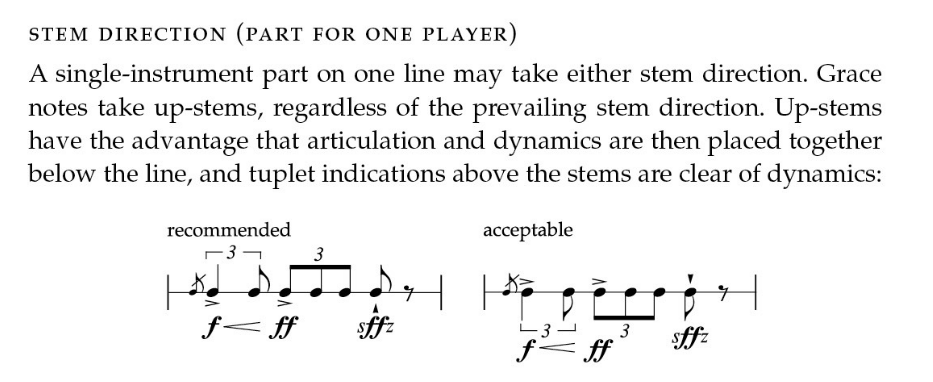
\includegraphics[height=40mm, width=90mm]{images/hampes_0.png} \\\textit{Source : Behind Bars, Elaine Gould}\\\\
Le principe ci-dessus semble être respecté dans les rythmiques binaires de Juskowiac mais pas dans les Méthodes agostini\\
—————————————————————————————————————————————————————————————————————————————————————